%\documentclass{article}
%
%\usepackage{fancyhdr}
%\usepackage{extramarks}
%\usepackage{amsmath}
%\usepackage{amsthm}
%\usepackage{amsfonts}
%\usepackage{tikz}
%\usepackage{enumerate}
%\usepackage{graphicx}
%\graphicspath{ {images/} }
%\usepackage[plain]{algorithm}
%\usepackage{algpseudocode}
%\usepackage[document]{ragged2e}
%\usepackage{textcomp}
%\usepackage{color}   %May be necessary if you want to color links
%\usepackage{import}
%\usepackage{hyperref}
%\hypersetup{
%    colorlinks=true, %set true if you want colored links
%    linktoc=all,     %set to all if you want both sections and subsections linked
%    linkcolor=black,  %choose some color if you want links to stand out
%}
%
%\usetikzlibrary{automata,positioning}
%
%
%% Basic Document Settings
%
%
%\topmargin=-0.45in
%\evensidemargin=0in
%\oddsidemargin=0in
%\textwidth=6.5in
%\textheight=9.0in
%\headsep=0.25in
%\setlength{\parskip}{1em}
%
%\linespread{1.1}
%
%\pagestyle{fancy}
%\lhead{\hmwkAuthorName}
%\lfoot{\lastxmark}
%\cfoot{\thepage}
%
%\renewcommand\headrulewidth{0.4pt}
%\renewcommand\footrulewidth{0.4pt}
%
%\setlength\parindent{0pt}
%
%
%\newcommand{\hmwkTitle}{Math Review Notes---Real Analysis}
%\newcommand{\hmwkAuthorName}{\textbf{G. Faletto} }
%
%
%%%%%% Title Page
%
%
%\title{
%    \vspace{2in}
%    \textmd{\textbf{ \hmwkTitle}}\\
%}
%
%\author{Gregory Faletto}
%\date{}
%
%\renewcommand{\part}[1]{\textbf{\large Part \Alph{partCounter}}\stepcounter{partCounter}\\}
%
%
%%%%%% Various Helper Commands
%
%
%%%%%% Useful for algorithms
%\newcommand{\alg}[1]{\textsc{\bfseries \footnotesize #1}}
%
%%%%%% For derivatives
%\newcommand{\deriv}[2]{\frac{\mathrm{d} #1}{\mathrm{d} #2}}
%
%%%%%% For partial derivatives
%\newcommand{\pderiv}[2]{\frac{\partial #1}{\partial #2}}
%
%%%%%% Integral dx
%\newcommand{\dx}{\mathrm{d}x}
%
%%%%%% Alias for the Solution section header
%\newcommand{\solution}{\textbf{\large Solution}}
%
%%%%%% Probability commands: Expectation, Variance, Covariance, Bias
%\newcommand{\E}{\mathbb{E}}
%\newcommand{\Var}{\mathrm{Var}}
%\newcommand{\Cov}{\mathrm{Cov}}
%\newcommand{\Bias}{\mathrm{Bias}}
%\newcommand\indep{\protect\mathpalette{\protect\independenT}{\perp}}
%\def\independenT#1#2{\mathrel{\rlap{$#1#2$}\mkern2mu{#1#2}}}
%\DeclareMathOperator{\Tr}{Tr}
%
%\theoremstyle{definition}
%\newtheorem{theorem}{Theorem}
%\theoremstyle{definition}
%\newtheorem{proposition}[theorem]{Proposition}
%\theoremstyle{definition}
%\newtheorem{lemma}[theorem]{Lemma}
%\theoremstyle{definition}
%\newtheorem{corollary}{Corollary}[theorem]
%\theoremstyle{definition}
%\newtheorem{definition}{Definition}[section]
%\newtheorem*{remark}{Remark}
%\theoremstyle{definition}
%\newtheorem{exercise}{Exercise}
%
%%%%%% Tilde
%\newcommand{\textapprox}{\raisebox{0.5ex}{\texttildelow}}
%
%\begin{document}
%
%\maketitle
%
%\pagebreak
%
%\tableofcontents
%
%\
%
%\
%
%\begin{center}
%Last updated \today
%\end{center}
%
%
%
%\newpage
%
%%
%%
%%
%%
%%
%%
%%
%%
%%%
%% Real Analysis

% Real Analysis
\section{Real Analysis}

These are my notes from Math 4650: Analysis I at Cal State LA as well as Prof. Steven Heilman's notes from Math 541A at USC.

%\textbf{Brush up on recent real analysis (especially open, closed, compact, etc)}

%Midterm 1
\subsection{Midterm 1}

% Homework 1
\subsubsection{Homework 1}

\begin{definition} Let \(S \subseteq \mathbb{R}\). We say that \(S\) is \textbf{bounded from above} if \(\exists \ b \in \mathbb{R}\) where \[s \leq b \ \forall \ s \in S\]If this is the case, we call \(b\) an \textbf{upper bound} of \(S\).

If \(b \leq c \) for all upper bounds \(c\) of \(S\), we call \(b\) the \textbf{supremum} of \(S\): \(b = \sup(S)\).

\end{definition}

\begin{definition} We say that \(S\) is \textbf{bounded from below} if \(\exists \ a \in \mathbb{R}\) where \[s \geq a \ \forall \ s \in S\]If this is the case, we call \(a\) a \textbf{lower bound} of \(S\).

If \(a \geq d \) for all lower bounds \(d\) of \(S\), we call \(a\) the \textbf{infimum} of \(S\): \(a = \inf(S)\).
\end{definition}

\begin{proposition} \textbf{Useful Sup/Inf Fact:} Let \(S \in \mathbb{R}\), \(S \neq \emptyset\). 

\begin{enumerate}[(1)]

\item Suppose \(S\) is bounded from above by an element \(b\). Then \(b = \sup(S) \iff \forall \ \epsilon >0 \ \exists \ x \in S\) with \[b - \epsilon < x \leq b\]

\item Suppose \(S\) is bounded from below by an element \(a\). Then \(a = \inf(S) \iff \forall \ \epsilon >0 \ \exists \ x \in S\) with \[a \leq x < a + \epsilon\]

\end{enumerate}

\end{proposition}

\textbf{Completeness Axiom}: Let \(S\) be a nonempty subset of \(\mathbb{R}\). If \(S\) is bounded from above, then \(\sup(S)\) exists. If \(S\) is bounded from below, then \(\inf(S)\) exists.

%\[
%|x - y| < \epsilon \iff y - \epsilon < x < y + \epsilon
%\]

\textbf{Facts about absolute value:}

\begin{itemize}

\item \begin{proposition}\label{ra.abs.fact1} \(|x-y| < \epsilon \iff y - \epsilon < x < y + \epsilon.\) \end{proposition}

\begin{proof}In notes 08/23.\end{proof}

\item \begin{proposition} \( |ab| = |a||b|. \)\end{proposition}

\begin{proof} \[| ab | = \begin{cases} 
      ab & ab \geq 0 \\
      -ab & ab < 0 
   \end{cases} = \begin{cases} 
      ab & a \geq 0,  b \geq 0 \\
      -ab & a \geq 0, b < 0 \\ 
      -ab & a < 0, b \geq 0 \\ 
      ab & a < 0,  b < 0 \\
   \end{cases} = \begin{cases} 
      ab & a \geq 0,  b \geq 0 \\
      a(-b) & a \geq 0, b < 0 \\ 
      (-a)b & a < 0, b \geq 0 \\ 
      (-a)(-b) & a < 0,  b < 0 \\
   \end{cases}
\]


\[= \begin{cases} 
      |a||b| & a \geq 0,  b \geq 0 \\
      |a||b| & a \geq 0, b < 0 \\ 
      |a||b| & a < 0, b \geq 0 \\ 
      |a||b| & a < 0,  b < 0 \\
   \end{cases} \implies | ab | = |a||b| 
\]

\end{proof}

\item \begin{proposition} Let \(\epsilon >0\). Then \(|a| < \epsilon \iff -\epsilon < a < \epsilon\). \end{proposition}

\begin{proof} Follows from Proposition \ref{ra.abs.fact1} if \(x = a\), \(y = 0\). \end{proof}

\item \begin{proposition} \(-|a| \leq a \leq |a|\)  \end{proposition}

\begin{proof}  Follows from Proposition \ref{ra.abs.fact1} if \(x = a\), \(y = 0\), \(\epsilon = |a|\). \end{proof}

\item \begin{theorem}\label{ra.tri.ineq.1} \textbf{Triangle Inequality:} \(|a + b| \leq |a| + |b|\). \end{theorem}

\begin{proof} In notes 08/23.\end{proof}

 \begin{corollary}\label{ra.tri.ineq.2} \textbf{Triangle Inequality:} \(|a - b| \leq |a| + |b|\). \end{corollary}

\begin{proof} Follows from Theorem \ref{ra.tri.ineq.1}, let \(b = -b\).

\end{proof}

\begin{remark} See also Theorem \ref{asym.tri.ineq.norm}.\end{remark}

\item \begin{proposition} \(|\ |a| - |b| \ | \leq |a - b|\). \end{proposition}

\begin{proof} By Proposition \ref{ra.abs.fact1}, \(|\ |a| - |b| \ | \leq |a - b|\) if and only if

\begin{equation}\label{ra.proof.eqn1}
|b| - |a - b| \leq |a| \leq |b| + |a - b|
\end{equation}

The left half of (\ref{ra.proof.eqn1}) is true by the Triangle Inequality (Theorem \ref{ra.tri.ineq.1}):

\[
|b| = |a - (a - b)| \leq |a| +  |a - b| \iff |b| \leq |a| +  |a - b| \iff  |b| - |a - b| \leq |a|
\]

The right half of  (\ref{ra.proof.eqn1}) is also true by the Triangle Inequality (Theorem \ref{ra.tri.ineq.1}):

\[
|a| = |b + a - b| \leq |b| + |a - b|
\]

Therefore

\[
|\ |a| - |b| \ | \leq |a - b|.
\] \end{proof}

\begin{proof}(Alternative proof.) Note that by the Triangle Inequality (Theorem \ref{ra.tri.ineq.1}),

\[
|a| = |a - b +b| \leq |a - b| + |b| \implies |a| - |b| \leq |a - b|
\]

Also,

\[
|b| = |b - a + a| \leq |b - a| + |a| \implies -|b - a| \leq |a| - |b| \implies -|a - b| \leq |a| - |b|
\]

where the last step follows from Proposition \ref{ra.abs.fact.a}. Therefore

\[
-|a - b| \leq |a| - |b| \leq |a - b|
\]

and by Proposition \ref{ra.abs.fact1},

\[
|\ |a| - |b| \ | \leq |a - b|.
\]
\end{proof}

\item \begin{proposition} If \(a < x < b\) and \(a < y < b\) then \(|x - y| < b - a\). \end{proposition}

\begin{proof}
\[
y > a \implies -y < -a \implies b - y < b - a
\]

\[
b > y \implies b - y = |b - y| \implies  \boxed{|b - y| < b - a}
\]

By the Triangle Inequality (Theorem \ref{ra.tri.ineq.1}),

\[
|x - y| = |x - b + b - y| \leq |x -b| + |b - y|
\]

Since \(b <x\), \(|x - b| > 0\). Therefore \(\boxed{|x - y| < | b - y|}\).

\[
\implies |x - y| < |b - y| < b - a
\]

\[
\implies |x - y| < b - a
\]
\end{proof}

\begin{proof} (Alternative proof.) Break into two cases.

\begin{itemize}

\item \textbf{Case 1:} \(x \geq y\). Then \(|x - y| = x - y\). We know \(a < x < b \implies 0 < x - a < b - a\). 

\[
a < y \implies -a > -y \implies x - a > x -y \implies x - y < x - a < b - a
\]

\[
\implies \boxed{|x - y| < b - a}
\]


\item \textbf{Case 2:} \(x < y\). Then \(|x - y| = y - x\). We know \(a < y < b \implies 0 < y - a < b - a\).

\[
a < x \implies -a > -x \implies y - a > y - x \implies y - x < y - a < b - a
\]

\[
\implies \boxed{|x - y| < b - a}
\]

\end{itemize}

\end{proof}

\item \begin{proposition}\label{ra.abs.fact.a} \(|a - b| = |b - a|\) \end{proposition}

\begin{proof} \(|a - b| = |(-1)(b - a)| = |-1||b-a| = |b - a|\), where the second-to-last step follows from Proposition \ref{ra.abs.fact1}.

\end{proof}

\end{itemize}

% Homework 2
\subsubsection{Homework 2}

\begin{definition}  A sequence \((a_n)\) of real numbers is said to \textbf{converge} to a \textbf{limit} \(L \in \mathbb{R}\) if \(\forall \ \epsilon > 0 \ \exists \ N > 0 \) where

\[
n \geq N \implies |a_n - L| < \epsilon
\]

We say that \((a_n)\) \textbf{diverges} if it does not converge.

\end{definition}

\begin{definition} A sequence \((a_n)\) of real numbers is \textbf{bounded} if \(\exists \ M > 0\) where \(\forall \ n \in \mathbb{N}\) \[\ |a_n| \leq M .\]

\end{definition}

\begin{theorem} If \((a_n)\) converges then \((a_n)\) is bounded. \end{theorem}

\begin{definition} Let \((a_n)\) be a sequence of real numbers. We say that \((a_n)\) is a \textbf{Cauchy sequence} if \(\forall \ \epsilon > 0 \ \exists \ N\) where

\[
n, m \geq N \implies |a_n - a_m| < \epsilon
\]

\end{definition}

\begin{theorem} \((a_n)\) is Cauchy if and only if \((a_n)\) converges.

\end{theorem}

\begin{corollary} If \((a_n)\) is Cauchy then \((a_n)\) is bounded.

\end{corollary}

%\begin{theorem} Suppose that \(\{a_n\}\) is a Cauchy sequence. Then \(\{a_n\}\) is bounded. \end{theorem}

\begin{proof} Let \(\epsilon = 1\). Since \((a_n)\) is Cauchy, \(\exists \ N > 0 \ | \ n, m \geq N \implies \)

\[
|a_n - a_m| < 1
\]

So, \(n \geq N \implies\)

\[
|a_n - a_N| < 1 \iff a_N - 1 < a_n < a_N + 1 \implies |a_n| < |a_N + 1| \leq |a_N| + 1
\]

Let \(M = \max \{ |a_1|, |a_2|, \ldots, |a_{N-1}|, |a_N| + 1\} \). Then \(|a_n| \leq  M \ \forall \ n \geq 1 \). Therefore \((a_n)\) is bounded.

\end{proof}

%\end{theorem}

\begin{theorem} \textbf{(Squeeze theorem.)} Suppose that \(\{a_n\}, \{b_n\},\) and \(\{c_n\}\) are sequences of real numbers such that \(a_n \leq b_n \leq c_n\) for all \(n\). If both \(\{a_n\}\) and \(\{c_n\}\) converge to \(L\), then \(\{b_n\}\) converges to \(L\).

\end{theorem}

\begin{proof} Let \(\epsilon >0\). \((a_n)\) converges to \(L \implies\)

\[
\forall \ \epsilon> 0 \ \exists \ N_A \ | \ n \geq N_A \implies | a_n - L | < \epsilon 
\]

\((c_n)\) converges to \(L \implies\)

\[
\forall \ \epsilon> 0 \ \exists \ N_C \ | \ n \geq N_C \implies | c_n - L | < \epsilon 
\]

Let \(N = \max \{N_A, N_C\} \). Then by one of our absolute values rules, \(n \geq N \implies\)

\[
| a_n - L | < \epsilon \iff L - \epsilon < a_n < L + \epsilon
\]

\[
| c_n - L | < \epsilon \iff L - \epsilon < c_n < L + \epsilon
\]

Therefore since \(a_n \leq b_n \leq c_n\),

\[
 L - \epsilon < a_n \leq b_n \leq c_n < L + \epsilon \implies L - \epsilon < b_n < L + \epsilon \iff | b_n - L | < \epsilon
\]

Therefore \((b_n)\) converges to \(L\).

\end{proof}

\begin{theorem} Suppose that \(\{a_n\}\) and \(\{b_n\}\) are sequences of real numbers such that \(a_n \leq b_n\) for all \(n\). If \(\{a_n\}\) and \(\{b_n\}\) converge to \(A\) and \(B\) respectively, then \(A \leq B\).

\end{theorem}

\begin{proof} Suppose \(A > B\). Then let \(\epsilon = \frac{A - B}{4} > 0\). \((a_n)\) converges to \(A \implies\)

\[
\exists \ N_A \ | \ n \geq N_A \implies | a_n - A | < \epsilon \iff A - \epsilon < a_n < A + \epsilon
\]

\((b_n)\) converges to \(B \implies\)

\[
\exists \ N_B \ | \ n \geq N_B \implies | b_n - B | < \epsilon \iff B - \epsilon < b_n < B + \epsilon
\]

Then if \(n > \max \{ N_A, N_B\} \),

\[
A - \epsilon < a_n < A + \epsilon \iff A - \frac{A - B}{4} < a_n < A +\frac{A - B}{4} \iff \frac{3A}{4} + \frac{B}{4} < a_n <  \frac{5A}{4} - \frac{B}{4}
\]

\[
B - \epsilon < b_n < B + \epsilon \iff B -\frac{A - B}{4}< b_n < B+ \frac{A - B}{4} \iff \frac{5B}{4} - \frac{A}{4} < b_n <  \frac{3B}{4} + \frac{A}{4}
\]

This implies

\[
 b_n <  \frac{3B}{4} + \frac{A}{4} = \frac{B}{4} + \frac{A}{4} + \frac{2B}{4} < \frac{B}{4} + \frac{A}{4} + \frac{2A}{4}  = \frac{3A}{4} + \frac{B}{4} < a_n
\]

Contradiction, since it is given that \(a_n \leq b_n \ \forall \ n\). Therefore \(A \leq B\).
\end{proof}

\pagebreak

% Midterm 2
\subsection{Midterm 2}

% Homework 3
\subsubsection{Homework 3}

\begin{definition} \textbf{(Limits of functions at infinity.)} Let \(f\) be a real-valued function defined on some set \(D\) where \(D\) contains an interval of the form \((a, \infty)\). Let \(L \in \mathbb{R}\). We say \[\lim_{x \to \infty} f(x) = L\]if \(\forall \ \epsilon >0 \ \exists \ N \in \mathbb{R}\) where

\[
x \geq N \implies |f(x) - L| < \epsilon.
\]

\end{definition}

\begin{definition}\label{ra.def.limit.point} Let \(D \subseteq \mathbb{R}\). Let \(a \in \mathbb{R}\). We say that \(a\) is a \textbf{limit point} (or ``cluster point," or ``accumulation point") of \(D\) if \(\forall \ \delta > 0 \ \exists \ x \in D\) where

\[
x \neq a \text{ and } |x - a| < \delta
\]

(Note that \(a\) may or may not be contained in \(D\).)

\end{definition}

\begin{definition} \textbf{(Limit of a function at \(a\).)}: Let \(D \subseteq \mathbb{R}\) and \(f:d \to \mathbb{R}\). Let \(a\) be a limit point of \(D\). Let \(x \in D\). We say that \(f\) has a \textit{limit as \(x\) tends to \(a\)} if \(\exists \ L \in \mathbb{R}\) where \(\forall \ \epsilon > 0 \ \exists \ \delta > 0 \) such that

\[
0 < |x - a| < \delta \implies |f(x) - L| < \epsilon
\]

and we write \[\lim_{x \to a} f(x) = L\]

\end{definition}

\begin{proposition} \textbf{(Properties of Limits.)} Let \(D \in \mathbb{R}\) and let \(a\) be a limit point of \(D\). Suppose \(f:D \to \mathbb{R}\) and \(g: D \to \mathbb{R}\). Let \(\alpha \in \mathbb{R}\).

\begin{enumerate}[(1)]

\item If \(\lim_{x \to a} f(x) = L\) and \(\lim_{x \to a} g(x) = M\) then

\begin{enumerate}[(a)]

\item \[\lim_{x \to a} \alpha = \alpha\]

\item \[\lim_{x \to a} [f(x) + g(x)] = L + M\]

\item \[\lim_{x \to a} [f(x) - g(x)] = L - M\]

\item \[\lim_{x \to a} [f(x) \cdot g(x)] = L \cdot M\]

\item \[\lim_{x \to a} [\alpha \cdot f(x)] = \alpha \cdot L\]

\end{enumerate}

\item If \(h:D \to \mathbb{R}\) and \(h(x) \neq 0 \ \forall \ x \in D\) and \(\lim_{x \to a} h(x) = H \neq 0\), then

\[
\lim_{x \to a} \frac{1}{h(x)} = \frac{1}{H}
\]

Note that properties (2) and (1)(d) combined imply

\[
\lim_{x \to a} \frac{f(x)}{h(x)} = \frac{L}{H}
\]

\end{enumerate}

\end{proposition}

% Homework 4
\subsubsection{Homework 4}

\begin{definition} \textbf{(Continuity.)} Let \(D \subseteq \mathbb{R}\) and \(f:D \to \mathbb{R}\) and \(a \in D\). Then \(f\) is \textbf{continuous} at \(a\) if \(\lim_{x \to a} f(x)\) exists and 

\[
\lim_{x \to a} f(x) = f(a)
\]

\end{definition}

\begin{remark} if \(f\) is continuous at \(a\), then we can say \(\forall \ \epsilon > 0 \ \exists \ \delta > 0 \) such that

\[
|x - a| < \delta \implies |f(x) - L| < \epsilon
\]

that is, we don't need to say \(0 < |x - a| < \delta\).

\end{remark}

\begin{definition} If \(B \subseteq D\), then \(f\) is \textbf{continuous on B} if \(f\) is continuous at every \(b \in B\).

\end{definition}

\begin{theorem} \textbf{(Intermediate Value Theorem.)} Let \(f\) be continuous on \([a, b]\) and suppose \(f(a) < f(b)\). \(\forall \ d\) such that \[f(a) < d < f(b)\]  \(\exists \ c \in \mathbb{R}\) where \[a < c < b, \ f(c) = d.\]

\end{theorem}

\pagebreak

% Final
\subsection{Final}

% Homework 5
\subsubsection{Homework 5}

\begin{definition} Let \(S \subseteq \mathbb{R}\). We say \(x \in \mathbb{R}\) is an \textbf{interior point} of \(S\) if there exists an open interval \((a, b)\) where \[x \in (a, b) \text{ and } (a, b) \subseteq S.\]

\end{definition}

\begin{definition} \textbf{(Open sets.)} Let \(S \subseteq \mathbb{R}\). We say \(S\) is \textbf{open} if every \(x \in S\) is an interior point of \(S\).

\end{definition}

\begin{definition} \textbf{(Closed sets.)} Let \(S \subseteq \mathbb{R}\). We say \(S\) is \textbf{closed} if \(\mathbb{R} \setminus S\) is open.

\end{definition}

\begin{theorem} A set is closed if and only if it contains all of its limit points.

\end{theorem}

\textbf{(Facts about open and closed sets.)} Suppose \(a, b \in \mathbb{R}\). Then

\begin{itemize}

\item \begin{proposition}\label{ra.hw5.5b} \((a, \infty)\) is open. \end{proposition}

\begin{proof} Let \(x \in (a, \infty)\). Since \(x > a\), \(\exists \ \epsilon >0 \ | \ a +  \epsilon = x\). Then \(a = x - \epsilon < x - \frac{\epsilon}{2} < x < x + \frac{\epsilon}{2} < \infty\). Therefore \(x \in (x - \frac{\epsilon}{2}, x + \frac{\epsilon}{2}) \subseteq (a, \infty)\), so \((a, \infty)\) is open. \end{proof}

\item \begin{proposition}\label{ra.hw5.5a} \((-\infty, b)\) is open. \end{proposition}

\begin{proof} Let \(x \in (-\infty, b)\). Since \(x < b\), \(\exists \ \epsilon >0 \ | \ b - \epsilon = x\). Then \(-\infty < x - \frac{\epsilon}{2} < x < x + \frac{\epsilon}{2} < x + \epsilon = b\). Therefore \(x \in (x - \frac{\epsilon}{2}, x + \frac{\epsilon}{2}) \subseteq (-\infty, b)\), so \((-\infty, b)\) is open. \end{proof}

\item \begin{proposition}\((a, b)\) is open. \end{proposition}

\begin{proof} In class notes. \end{proof}

\item \begin{proposition}\label{ra.hw5.5c} If \(a < b\), then \([a, b]\) is closed. \end{proposition} 

\begin{proof} Consider \(\mathbb{R} \setminus [a, b] = (-\infty, a) \cup (b, \infty)\). By Proposition \ref{ra.hw5.5a}, \((-\infty, a) \) is open. By Proposition {ra.hw5.5b}, \((b, \infty)\) is open. By Proposition \ref{ra.hw5.3b}, the union of two open sets is open. Therefore \(\mathbb{R} \setminus [a, b]\) is open, so \([a, b]\) is closed. \end{proof}

\item \begin{proposition}\label{ra.hw5.3b} If \(A\) and \(B\) are open, then \(A \cup B\) is open.  \end{proposition} 

\begin{proof} Since \(A\) is open, \(\forall \ x_A \in A \ \exists \ (a_A, b_A) \subseteq A \ | \ x_A \in (a_A, b_A)\). Since \(B\) is open, \(\forall \ x_B \in B \ \exists \ (a_B, b_B) \subseteq B \ | \ x_B \in (a_B, b_B)\). 

Let \(x \in A \cup B\). If \(x \in A\), then per above \( \exists \ (a_A, b_A) \subseteq A \subseteq A \cup B \ | \ x_A \in (a_A, b_A)\). If \(x \in B\), then per above \(\exists \ (a_B, b_B) \subseteq B \subseteq A \cup B \ | \ x_B \in (a_B, b_B)\). Therefore \(A \cup B\) is open.
\end{proof}

\item \begin{proposition}\label{ra.hw5.3a} If \(A\) and \(B\) are open, then \(A \cap B\) is open.  \end{proposition} 

\begin{proof} Since \(A\) is open, \(\forall \ x_A \in A \ \exists \ (a_A, b_A) \subseteq A \ | \ x_A \in (a_A, b_A)\). Since \(B\) is open, \(\forall \ x_B \in B \ \exists \ (a_B, b_B) \subseteq B \ | \ x_B \in (a_B, b_B)\).

Let \(x \in A \cap B\). Then \(x \in A\) and \(x \in B\), so \(\exists  \ (a_A, b_A) \subseteq A \ | \ x_A \in (a_A, b_A)\), and \(\exists \ (a_B, b_B) \subseteq B \ | \ x_B \in (a_B, b_B)\). Let \(a = \max \{a_A, a_B \}\), and \(b = \min \{b_A, b_B\} \). Since \(x > a\) and \(x < b\), \(x \in (a, b)\). Since \((a, b) \subseteq (a_A, b_A) \subseteq A\) and \((a, b) \subseteq (a_B, b_B) \subseteq B\), \((a, b) \subseteq A \cap B\). Therefore \(A \cap B\) is open. \end{proof}

\item \begin{proposition}\label{ra.hw5.4a} If \(A\) and \(B\) are closed, then \(A \cup B\) is closed. \end{proposition} 

\begin{proof} Since \(A\) is closed, \(\mathbb{R} \setminus A\) is open. Since \(B\) is closed, \(\mathbb{R} \setminus B\) is open. \(\mathbb{R} \setminus (A \cup B) = (\mathbb{R} \setminus A) \cap (\mathbb{R} \setminus B)\). By Proposition \ref{ra.hw5.3a} the intersection of two open sets is open. Therefore \(\mathbb{R} \setminus (A \cup B) \) is open, so \(A \cup B\) is closed.

\end{proof}

\item \begin{proposition}\label{ra.hw5.4a} If \(A\) and \(B\) are closed, then \(A \cap B\) is closed. \end{proposition} 

\begin{proof} Since \(A\) is closed, \(\mathbb{R} \setminus A\) is open. Since \(B\) is closed, \(\mathbb{R} \setminus B\) is open. \(\mathbb{R} \setminus (A \cap B) = (\mathbb{R} \setminus A) \cup (\mathbb{R} \setminus B)\). By Proposition \ref{ra.hw5.3b}, the union of two open sets is open. Therefore \(\mathbb{R} \setminus (A \cap B) \) is open, so \(A \cap B\) is closed.

\end{proof}

\item \begin{proposition}\label{ra.hw5.1} \(\mathbb{R}\) is open and closed. \end{proposition}

\begin{proof} Let \(\epsilon > 0\). Let \(x \in \mathbb{R}\). Then \(x - \epsilon, x + \epsilon \in \mathbb{R}\), and \(x \in (x - \epsilon, x + \epsilon)\). Therefore \(\mathbb{R}\) is open. \(\mathbb{R}\) is closed because by Proposition \ref{ra.hw5.2}, \(\mathbb{R} \setminus \mathbb{R} = \emptyset\) is open. \end{proof}

\item \begin{proposition}\label{ra.hw5.2} \(\emptyset\) is open and closed. \end{proposition}

\begin{proof} To show that a set \(S\) is open, we most show that \(\forall \ x \in  S \ \exists \ S' \subseteq S | \ x \in S' \) where \(S'\) is open. Since there are no \(x \in \emptyset\), this condition is satisfied for \(\emptyset\). \(\emptyset\) is closed because per Proposition \ref{ra.hw5.1}, \(\mathbb{R} \setminus \emptyset = \mathbb{R}\) is open.

\end{proof}

\end{itemize}

\begin{proposition}\label{ra.hw5.6a} Let \(x_1, x_2, \ldots, x_n\) be real numbers. Let \(S\) be the finite set \(S = \{x_1, x_2, \ldots, x_n\}\). Then \(S\) is closed.\end{proposition}

\begin{proof} Consider \(\mathbb{R} \setminus S = (-\infty, x_1) \cup (x_1, x_2) \cup \ldots \cup (x_{n-1}, x_n) \cup (x_n, \infty)\). \((-\infty, x_1)\) is open by Proposition \ref{ra.hw5.5a}. \((x_n, \infty)\) is open by Proposition \ref{ra.hw5.5b}. 

Consider \((x_i, x_{i+1})\) where \(i \in \{1, 2, 3, \ldots, n-1\}\). Let \(x \in (x_i, x_{i+1})\). Then since \(x > x_i\) and \(x < x_{i+1}\), \(\exists \ \epsilon > 0 \ | \ x_i + \epsilon = x\) and \(\exists \ \delta > 0 \ | \ x_{i+1} - \delta = x\). Then \(x_i = x - \epsilon < x - \frac{\epsilon}{2} < x < x + \frac{\delta}{2} < x + \delta = x_{i+1}\). Therefore \(x \in (x - \epsilon, x + \delta) \subseteq (x_i, x_{i+1})\), so \((x_i, x_{i+1})\) is open.

Finally, since \(\mathbb{R} \setminus S\), by Proposition \ref{ra.hw5.5b} (and induction) \(\mathbb{R} \setminus S\) is open. Therefore \(S\) is closed.
\end{proof}

\begin{proposition}\label{ra.hw5.6b} Let \(x_1, x_2, \ldots, x_n\) be real numbers. Let \(S\) be the finite set \(S = \{x_1, x_2, \ldots, x_n\}\). Then \(S\) has no limit points.\end{proposition}

\begin{proof} 

%\textbf{Limit point:} Let \(D \subseteq \mathbb{R}\). We say that \(a\) is a \textit{limit point} of \(D\) if \(\forall \ \delta >0 \ \exists \ x \in D\) with \(x \neq a, |x - a| < \delta\). 

Per Definition \ref{ra.def.limit.point}, we seek to show that (1) \(\forall \ x_i \in S \ \exists \ \delta_i\) such that \(\forall \ x_j \in D (x_j \neq x_i)\) \[|x_j - x_i| \geq \delta_i\] and (2) \(\forall \ x \in \mathbb{R} \setminus S \ \exists \ \delta_x\) such that \(\forall \ x_i \in D\) \[|x_i - x| \geq \delta_x\]

\begin{enumerate}[(1)]
\item Let \(x_i \in S\). Let \(\delta_i = \frac{1}{2}\min \{|x_i - x_k| \ | \ x_k \neq x_i \}\). Then \(\forall \ x_j \neq x_i \in S\), 

\[
|x_i - x_j| \geq |x_i - x_k| > \delta_i
\]

\item Let \(x \in \mathbb{R} \setminus S\). Let \(\delta_x = \frac{1}{2} \min \{|x - x_i| \ | \ x_i \in S \} \). Then

\[
|x_i - x| \geq  \min \{|x - x_i| \ | \ x_i \in S \} > \delta_x
\]

\end{enumerate}
\end{proof}

\begin{definition} Let \(S \subseteq \mathbb{R}\). An \textbf{open cover} of \(S\) is a collection \(X = \{\mathcal{O}_\alpha \ | \ \alpha \in I \} \) where each set \(\mathcal{O}_\alpha\) is an open subset of \(\mathbb{R}\) such that

\[
S \subseteq \bigcup_{\alpha \in I} \mathcal{O}_\alpha
\]

(Here \(I\) is some set that indexes the \(\mathcal{O}_\alpha\)).

\end{definition}

\begin{definition} If \(X' \subseteq X\) such that \[S \subseteq  \bigcup_{\mathcal{O}_\alpha \in X'} \mathcal{O}_\alpha\]then \(X'\) is called a \textbf{subcover} of \(S\) contained in \(X\). In addition, if \(X'\) is finite then we call \(X'\) a \textbf{finite subcover} of \(S\) contained in \(X\).

\end{definition}

\begin{definition} \textbf{(Compactness.)} Let \(S \subseteq \mathbb{R}\). We say that \(S\) is \textbf{compact} if every open cover of \(S\) contains a finite subcover. 

\end{definition}

\begin{definition} Let \(S \subseteq \mathbb{R}\). We say that \(S\) is \textbf{bounded} if \(\exists \ M > 0\) where \(S \subseteq [-M, M]\).

\end{definition}

\begin{remark} \(S\) is bounded if and only if \(|s| \leq M\  \forall \ s \in S \).

\end{remark}

\begin{theorem}\label{ra.heine-borel.thm} \textbf{(Heine-Borel Theorem.)} Let \(S \subseteq \mathbb{R}\). \(S\) is compact if and only if \(S\) is closed and bounded.

\end{theorem}

\begin{proposition}\label{ra.hw6.1} Let \(x_1, x_2, \ldots, x_n\) be real numbers. Let \(S\) be the finite set \(S = \{x_1, x_2, \ldots, x_n\}\). Then \(S\) is compact.\end{proposition}

\begin{proof} Let \(\{O_\alpha\}\) be an open cover of \(S\). By definition of open cover, \(\forall \ i \ \exists \ O_{\alpha_i}\) such that \(x_i \in O_{\alpha_i}\). Thus, \( \{O_{\alpha_1}, O_{\alpha_2}, \ldots, O_{\alpha_n} \} \) is a finite subcover of \(S\). \end{proof}
%\pagebreak

\begin{proposition}\label{ra.hw6.5a} Let \(A\) and \(B\) be compact subsets of \(\mathbb{R}\). Then \(A \cap B\) is compact. \end{proposition}

\begin{proof} Since \(A \cap B \subseteq A\), \(A \cap B \subseteq [-M_A, M_A]\). Therefore \(A \cap B\) is bounded.

Since \(A \cap B\) is closed and bounded, by the Heine-Borel Theorem (Theorem {ra.heine-borel.thm}), \(A \cap B\) is compact.

\end{proof}

\begin{proposition}\label{ra.hw6.5b} Let \(A\) and \(B\) be compact subsets of \(\mathbb{R}\). Then \(A \cup B\) is compact. \end{proposition}

\begin{proof} Let \(M = \max \{ M_A, M_B \} \). Note that \([-M_A, M_A] \subseteq [M, M]\) and \([-M_B, M_B] \subseteq [-M, M]\). This implies \(A \subseteq [-M, M]\) and \(B \subseteq [-M, M]\). Therefore \(A \cup B \subseteq [-M, M]\).

Since \(A \cup B\) is closed and bounded, by the Heine-Borel Theorem (Theorem {ra.heine-borel.thm}), \(A \cup B\) is compact.

\end{proof}

\begin{theorem} Let \(f: D \to \mathbb{R}\) be continuous on \(D\). If \(X \subseteq D\) and \(X\) is compact (closed and bounded), then

\[
f(\bar{x}) = \{f(x) \ | \ x \in X\}
\]

is compact (closed and bounded).

\end{theorem}

\begin{corollary} Suppose \(f: D \to \mathbb{R}\) where \(D\) is closed and bounded. Then there exists \(a, b \in D\) where \(f(a)\) is the min of \(f\) on \(D\) and \(f(b)\) is the max of \(f\) on \(D\).

\end{corollary}

% Homework 6
\subsubsection{Homework 6}

\begin{definition} \textbf{(Uniform Continuity.)} Let \(D \subseteq \mathbb{R}\) and let \(f: D \to \mathbb{R}\). We say that \(f\) is \textbf{uniformly continuous} on \(D\) if \(\forall \ \epsilon > 0 \ \exists \ \delta > 0\) where

\[
x, y \in D \text{ and } 0 < |x - y| < \delta \implies |f(x) - f(y)| < \epsilon
\]

\end{definition}

\begin{theorem} \textbf{(Uniform continuity implies continuity.)} Suppose \(f:D \to \mathbb{R}\) where \(D \subseteq \mathbb{R}\). If \(f\) is uniformly continuous on \(D\), then \(f\) is continuous at every \(a \in D\).

\end{theorem}

\subsection{More Theorems}

\begin{theorem}\label{ra.fubini} \textbf{Fubini's Theorem.} Let \(h: \mathbb{R}^2 \to \mathbb{R}\) be a continuous function such that \(\int \int_{\mathbb{R}^2}|h(x,y)| dxdy < \infty\). Then

\[
\int \int_{\mathbb{R}^2} h(x,y)dxdy = \int_{\mathbb{R}} \bigg( \int_{\mathbb{R} } h(x,y)dx \bigg) dy = \int_{\mathbb{R}} \bigg( \int_{\mathbb{R}} h(x,y)dy \bigg) dx
\]

\end{theorem}

\subsection{Problems from Practice Math GRE Subject Tests}

%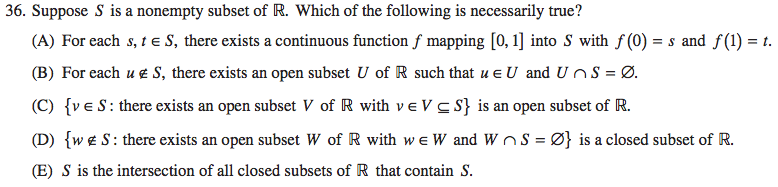
\includegraphics[scale=0.65]{1268_36}
%
%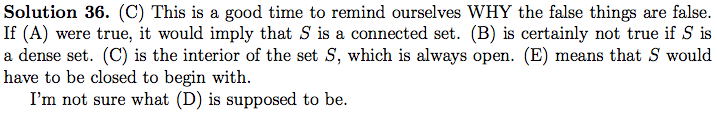
\includegraphics[scale=0.65]{1268_36s}

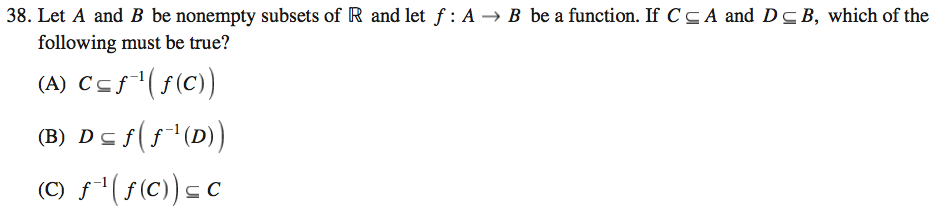
\includegraphics[scale=0.5]{0568_38}

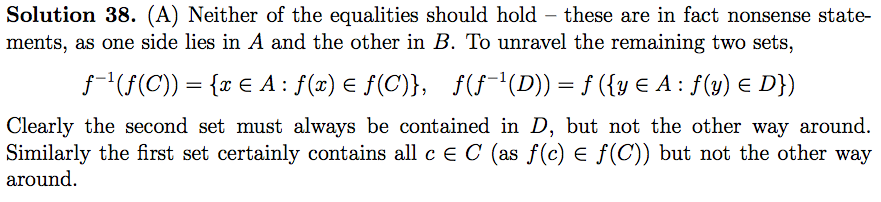
\includegraphics[scale=0.5]{0568_38s}

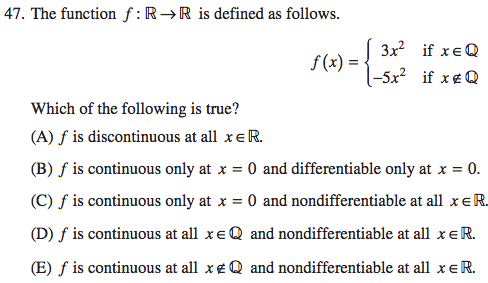
\includegraphics[scale=0.65]{1268_47}

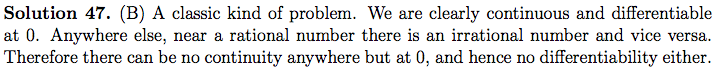
\includegraphics[scale=0.65]{1268_47s}

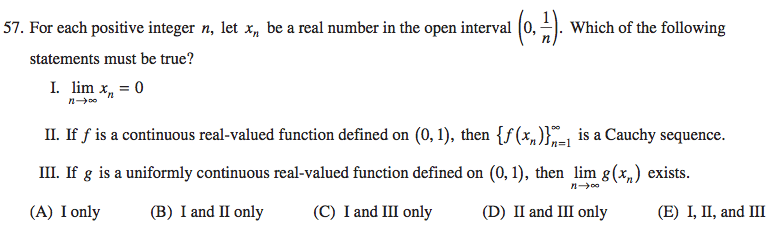
\includegraphics[scale=0.65]{1268_57}

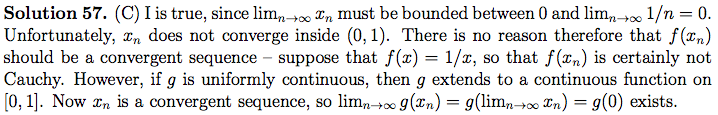
\includegraphics[scale=0.65]{1268_57s}

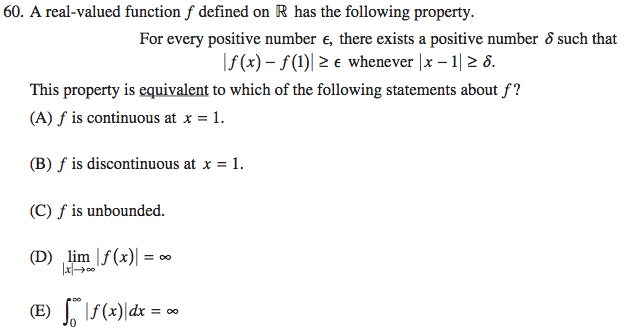
\includegraphics[scale=0.65]{1268_60}

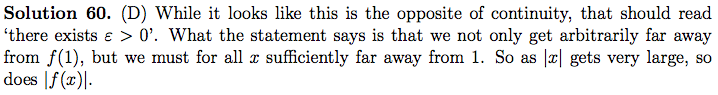
\includegraphics[scale=0.65]{1268_60s}

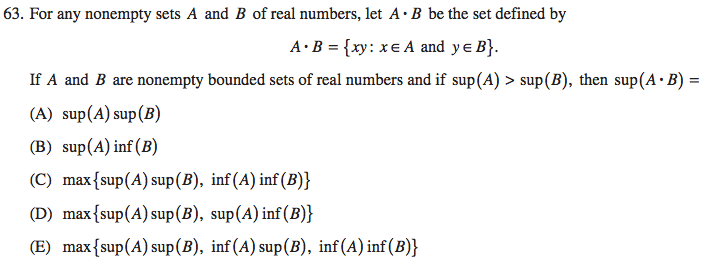
\includegraphics[scale=0.65]{1268_63}

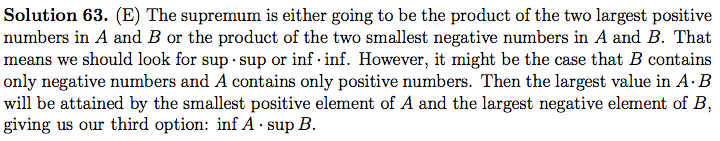
\includegraphics[scale=0.65]{1268_63s}

%\end{document}